\documentclass[11pt,a4paper]{article}

% Journal-neutral submission build for JAIR.
% IMPORTANT: Before portal upload, replace this preamble with the official
% JAIR Author Kit (ACM-based) from https://www.jair.org/index.php/jair/formatting
% and merge the reproducibility checklist from that kit.

\usepackage[margin=1in]{geometry}
\usepackage{graphicx}
\usepackage{booktabs}
\usepackage{tabularx}
\usepackage{hyperref}
\usepackage{xcolor}
\usepackage{amsmath}
\usepackage{microtype}
\usepackage{fontspec}
\defaultfontfeatures{Ligatures=TeX}
\setmainfont{Times New Roman}
\setmonofont{Menlo}
\usepackage[authoryear,round,semicolon]{natbib}

\title{A Knowledge Representation Framework for Historical AI Decision Reconstruction}
\author{Monika Dvo\v{r}\'{a}\v{c}kov\'{a}\\
ORCID: \href{https://orcid.org/0009-0009-0879-1605}{0009-0009-0879-1605}\\
\textit{[Affiliation to be filled --- author confirmation required]}\\
Corresponding author: Monika Dvo\v{r}\'{a}\v{c}kov\'{a} (\texttt{[email to be filled]})}
\date{}

\begin{document}
\maketitle

\begin{abstract}
\textbf{Objective.}
We refine and characterize the historical decision reconstruction problem for AI systems as a knowledge-representation and AI-systems problem: recovering, as of decision time, the decision knowledge that identifies an AI-assisted Decision Episode and restates its justification, authorization, and temporal validity.

\textbf{Methods.}
We distinguish execution artefacts from decision knowledge, derive technology-neutral reconstruction requirements (Reconstruction Checklist), perform unit evaluation of thirteen representative infrastructure sources, and conduct compositional evaluation via adversarial scenarios and binding analysis. We differentiate the approach from decision provenance and from the Decision Evidence Maturity Model (DEMM).

\textbf{Findings.}
Reviewed infrastructure families are often capable for native purposes but do not jointly preserve sufficient decision knowledge under default composition without durable bindings to a shared Decision ID and decision-time versions (ecosystem base triad: FAIL). A derived Knowledge Continuity Model (KCM) instantiates the stated requirements under stated population and preservation assumptions (internal coverage: PASS under assumptions); this is not independent empirical confirmation.

\textbf{Conclusions.}
The principal contribution is a refined representational and compositional characterization of historical decision reconstruction requirements across heterogeneous AI infrastructure. KCM and the conformance specification are derived engineering responses. Selected representational objects are further instantiated in a reference implementation (AIGov) to demonstrate implementation feasibility---not independent validation of the theory. Legal and governance domains motivate and stress-test the problem but are not the scientific object.
\end{abstract}

\noindent\textbf{Keywords:} historical decision reconstruction; knowledge representation; decision knowledge; Decision Episode; semantic bindings; AI systems; compositional evaluation; Knowledge Continuity Model


\section*{Declarations}
\paragraph{Acknowledgements.}
\textit{[Author confirmation required.]} No acknowledgements text is recorded in the repository.

\paragraph{Funding.}
No specific external funding is recorded for this work in the repository. \textit{[Author confirmation required before submission.]}

\paragraph{Competing interests.}
The author declares that she has no competing interests of which the repository provides contrary evidence. \textit{[Author confirmation required before submission.]}

\paragraph{Author contributions.}
Conceptualization, investigation, formal analysis, writing --- Monika Dvo\v{r}\'{a}\v{c}kov\'{a}.

\paragraph{Data and artefact availability.}
Evaluation artefacts (unit reviews, coverage audit, scenarios, composition analysis, reconstruction checklist, Knowledge Continuity Model, and conformance specification) are maintained under \texttt{topics/ai-infrastructure-gap/} in the associated research repository. No separate experimental dataset was collected.

\paragraph{Code availability.}
A reference implementation (AIGov) is reported solely as a feasibility demonstration that selected representational objects can be instantiated; it is not evaluated as empirical validation of the theory. Editable figure sources (Mermaid and Graphviz) are included in the submission package.

\paragraph{Use of generative AI.}
\textit{[Author confirmation required.]} Any use of AI tools in manuscript preparation must be disclosed in accordance with JAIR policy. AI systems are not authors and must not be credited as such.


% Abstract handled in preamble
\section{Introduction}

\subsection{1.1 The AI problem: historical reconstruction of decision knowledge}

AI systems increasingly participate in decisions whose meaning depends on more than a final output label. An AI-assisted decision is typically the result of interacting components: model inference, input evidence, thresholds or rules, optional human acceptance or override, and the criteria treated as applicable at the moment of commitment. Months later---during debugging of decision quality, analysis of model drift, multi-agent handoff review, long-lived assistant audit trails, or operational incident analysis---a fundamental AI-systems question arises:


\begin{quote}
Can we reconstruct, from retained structure alone, \emph{what decision knowledge held at decision time}---not what the live system would compute now?
\end{quote}

In practice, AI deployments retain abundant \textbf{execution artefacts}: traces of how computation proceeded, logs that events occurred, provenance of how artefacts were derived, lineage of datasets and pipelines, and documentation of released models. These artefacts answer important questions about execution and derivation. They do not, by themselves, answer whether the system preserved a coherent \textbf{representation of the decision}: its identity, outcome, temporal anchor, governing criteria versions, relied-upon evidence, model participation, human interventions, and authority under which the outcome was committed.


The result is a characteristic failure mode of contemporary AI stacks. Policies, prompts, models, and features drift; live stores overwrite decision-time inputs; human overrides may leave only a final business state; explanations may be regenerated after the fact from a different model version. A reconstructor who consults ``what the system says now'' risks substituting present computational narrative for historical decision knowledge. This is a problem of \textbf{representation, semantic binding, and temporal persistence}---core concerns of knowledge representation, AI systems, autonomous agents, multi-agent systems, decision support, reasoning over historical state, explainability infrastructure, and long-lived AI systems---before it is a problem of any particular application domain.


\subsection{1.2 Why execution artefacts are not enough}

We distinguish \emph{execution artefacts} from \emph{decision knowledge}. Execution artefacts record paths, events, and derivations. Decision knowledge, for reconstructability, must represent at least: the decision as an identifiable episode; the outcome; the time and versioned context; the justification structure (evidence available versus relied upon, and participating AI outputs); the authorization structure (actors and authority relative to applicable criteria); and the validity structure (constraints and rules treated as in force, without silent latest-only substitution).


Adjacent AI capabilities are routinely mistaken for this representational target. Replay restores computational paths without necessarily restoring normative decision structure. Provenance can encode portions of historical decision knowledge and is a relevant representational substrate, yet provenance alone does not guarantee reconstruction of justification, authorization, temporal validity, actual reliance, or cross-component semantic bindings. Explainability often yields contemporaneous or regenerable accounts. Model reproducibility recreates outputs without reconstructing the criteria and authority under which an output became a committed decision. The research gap we pursue is therefore not the claim that logging, provenance, or explanation mechanisms are absent or that prior work ignored decisions. It is that heterogeneous AI-system components still lack a durable, compositional \textbf{representation of decision episodes} that binds those components into historically interpretable decision knowledge---an aspect previously under-characterized in this specific representational and compositional form.


\subsection{1.3 Problem statement: historical decision reconstruction}

We refine and formalize the \textbf{historical decision reconstruction problem} for Artificial Intelligence systems:


\begin{quote}
Given only retained structured information and a stated reconstruction procedure, recover---deterministically and as of decision time---the decision knowledge that identifies an AI-assisted decision episode and restates its justification, authorization, and temporal validity, without substituting current execution state for historical decision state.
\end{quote}

The problem is a \textbf{knowledge-representation and AI-systems} problem. It exists whenever AI components participate in committed outcomes whose basis must remain interpretable after drift, update, or redistribution of system state. It does \textbf{not} depend on law, regulation, governance, or compliance. Those regimes are application settings in which the same representational deficiency becomes externally visible; they do not define the problem.


\subsection{1.4 Related diagnostic work and differentiation from DEMM}

Prior work already addresses provenance of automated decisions, accountable decision pipelines, structured records of entities, activities, agents, and derivations, and explanations generated from retained provenance \citep{singh2019decisionProvenance,huynh2021provenanceExplanations,moreau2013provDm}. Governance-oriented evidence assessment likewise shares a diagnostic concern with our evaluation. The Decision Evidence Maturity Model (DEMM) \citep{solozobov2026demm} operationalises governance-evidence sufficiency through property-level reconstructability assessment. DEMM evaluates evidence produced by existing upstream systems and identifies the \emph{container fallacy}: the presence of evidence containers does not establish reconstructability. We share that diagnostic concern. Our primary research question differs: we characterize the \textbf{representational capability} that AI systems must preserve for faithful historical reconstruction. Our scientific object is historical decision knowledge represented through \textbf{Decision Episodes}; we derive decision-time preservation and binding requirements; we treat justification, authorization, and temporal validity as distinct reconstruction targets; we distinguish relied-upon evidence from merely available evidence; and we evaluate compositional sufficiency across heterogeneous infrastructure families. DEMM and this manuscript are related; neither subsumes the other. Section 2 expands this comparison.


\subsection{1.5 Motivating application domains}

The problem appears in long-lived decision-support systems; AI assistants that accumulate commitments; orchestrated multi-step AI workflows; autonomous systems whose acts must remain interpretable after model or criteria updates; and multi-agent systems in which evidence and authority cross agent boundaries. External scrutiny in regulated deployments---including record-keeping practices discussed under instruments such as the EU AI Act \citep{eu2024aiAct}---stress-tests the same deficiency. These domains motivate and illustrate; they are not the scientific object of the paper. The manuscript remains coherent if legal references are set aside.


\subsection{1.6 Research question and contributions}

This paper asks:


\begin{quote}
Can existing AI systems infrastructure for provenance, observability, metadata, policy, documentation, explanation, and human--AI interaction---alone or in composition---support deterministic faithful reconstruction of justification, authorization, and temporal validity for historically situated AI-assisted decisions; and if not, how should the missing representational capability be characterized and what minimum structures and semantic bindings does that characterization imply?
\end{quote}

We structure the answer so that engineering artefacts remain consequences of problem characterization:


\begin{enumerate}
\item \textbf{Refine} the historical decision reconstruction problem as a knowledge-representation and AI-systems formulation, with an explicit distinction between execution artefacts and decision knowledge.
\item \textbf{Characterize} representational requirements for historical decision knowledge (justification, authorization, temporal validity, reliance, and semantic bindings).
\item \textbf{Evaluate} contemporary AI infrastructure families at unit level against those requirements.
\item \textbf{Evaluate} compositional sufficiency across heterogeneous families (scenarios and composition analysis).
\item \textbf{Identify} the residual gap: missing durable semantic bindings and shared decision identity.
\item \textbf{Derive} an engineering response---the Knowledge Continuity Model (KCM) and a Conformance Specification---as consequences of that analysis; then evaluate the derived response on the same bar.
\end{enumerate}

\textbf{Principal scientific contribution.} A refined formulation and systematic characterization of the historical decision reconstruction problem---previously under-characterized in this specific representational and compositional form---including representational requirements and compositional evaluation of reconstructability.


\textbf{Derived engineering contribution.} The Decision Episode abstraction, KCM objects and semantic bindings, and conformance classes---as \emph{one} solution implied by the characterization, not as the paper's primary claim.


\textbf{What this paper is not.} It is not a new logging system, not a provenance serialization format, not a workflow engine, and not an explainability method. Nor is its principal contribution an architecture proposal for its own sake. Those mechanisms remain components; the characterized problem is whether AI systems represent historically reconstructable decisions with the bindings needed for compositional sufficiency.


We do not claim that reconstruction is metaphysically impossible everywhere, nor that only a branded product can succeed. We claim, on the basis of the completed evaluation, that the reviewed composition of AI-systems standards and frameworks does not guarantee deterministic faithful reconstruction without durable episode-centric representational bindings, and that the derived KCM information requirements appear sufficient for the base triad when those bindings are populated under stated assumptions.


Figure 1 summarizes the scientific narrative: execution preservation is widespread; decision-knowledge preservation remains under-characterized compositionally; requirements formalize the gap; evaluation diagnoses composition failure; KCM is derived as an engineering response and checked for internal requirement coverage on the same bar.


\begin{figure*}[t]
\centering
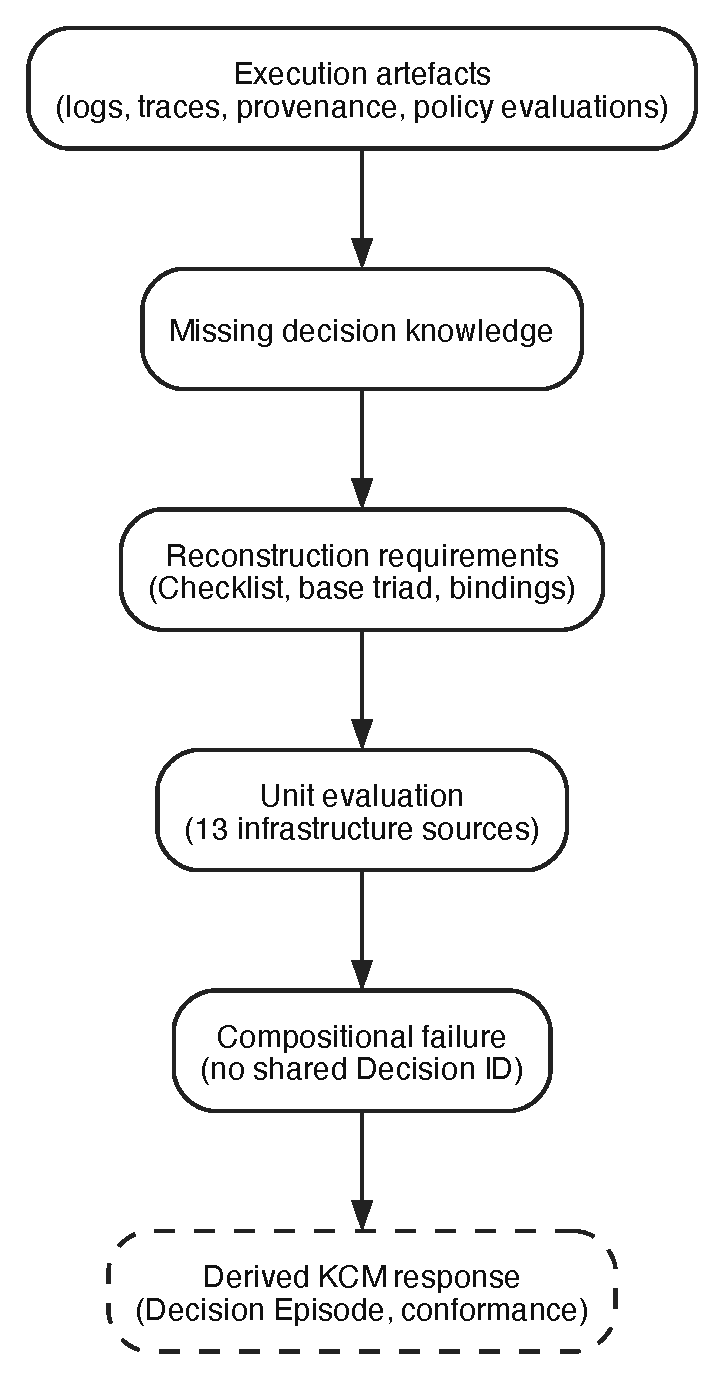
\includegraphics[width=\textwidth]{figures/fig1-scientific-argument.pdf}
\caption{Scientific argument: execution artefacts reveal missing decision knowledge; reconstruction requirements drive unit and compositional evaluation; the Knowledge Continuity Model is a \emph{derived} response, not the starting contribution. (Source: \texttt{figures/fig1-scientific-argument.pdf}.)}
\label{fig:1}
\end{figure*}

The remainder of the paper follows that narrative. Section 2 synthesizes related infrastructure, adjacent KR traditions, and differentiates DEMM and decision-provenance work. Section 3 formalizes reconstruction requirements. Section 4 describes evaluation methodology. Section 5 reports results on existing approaches. Section 6 derives the Knowledge Continuity Model. Section 7 summarizes the derived Conformance Specification. Section 8 evaluates the derived solution. Sections 9--11 discuss implications, threats, and conclusions.



\section{Related Work}

We organize related work by capability families evaluated in our unit reviews, then differentiate the strongest related diagnostic framing (DEMM) and clarify decision-provenance positioning. Each family contributes real AI-systems infrastructure. None---individually or by unspecified composition---defines a complete, durable \textbf{decision-episode representation} for base-triad reconstruction as characterized here. Table 1 summarizes the families; detailed checklist scores live in the unit reviews and are not repeated here.




\begin{table*}[t]
\centering
\small
\begin{tabularx}{\textwidth}{|X|X|X|X|X|}
\hline
 Family & Representative sources & Native strength & Reconstruction contribution & Principal limitation alone \\
 \hline
 \hline
 Provenance & W3C PROV-DM & Entities, activities, agents, derivation & Derivation and responsibility graphs & Not a shared Decision ID / reliance / policy-version episode model \\
 \hline
 Observability & OpenTelemetry & Traces, metrics, logs & Execution-path reconstructability & Paths $\neq$ normative decision structure; no standard Decision Episode semantic \\
 \hline
 ML metadata & Google ML Metadata & Artefacts, executions, contexts & Model/run heritage & Pipeline-centric; unbound to business Decision ID \\
 \hline
 Data lineage & OpenLineage & Job/dataset lineage & Feature/training heritage & Unbound to decision identity and reliance subset \\
 \hline
 Policy / authz & OPA; Cedar & Allow/deny eval; optional decision logs & Authorization \emph{islands} (esp. OPA bundle revision) & Cross-component episode binding absent; Cedar durability not mandated \\
 \hline
 Documentation & Model Cards; Datasheets; System Cards & Release-time transparency & Version/background knowledge & Cards describe releases, not sealed episode associations \\
 \hline
 Risk guidance & NIST AI RMF 1.0 & Organizational oversight processes & Process context & Process docs $\neq$ decision-time reconstruction schema \\
 \hline
 Explainability & NISTIR 8312 & Explanation quality principles & Clarifies explanation goals & Quality $\neq$ retained decision-bound justification package \\
 \hline
 Regulated logging & EU AI Act logging duties (motivating) & Retention-backed operational events & Monitoring stress-test & Not a cross-component Decision Episode contract \\
 \hline
 Human--AI workflow & OASIS WS-HumanTask & Task lifecycle, roles, history API & Human-gate acts & No mandated retention/rationale or shared Decision ID \\
 \hline
\end{tabularx}
\end{table*}


\subsection{2.1 Provenance and decision provenance}

W3C PROV-DM provides a normative vocabulary for entities, activities, agents, usage, generation, and derivation \citep{moreau2013provDm}. It systematically supports responsibility relations and time-stamped process graphs. Prior work already addresses provenance of automated decisions, accountable decision pipelines, structured records of entities, activities, agents, and derivations, and explanations generated from retained provenance---including decision-provenance and provenance-backed explanation lines of research \citep{singh2019decisionProvenance,huynh2021provenanceExplanations}. Provenance is therefore a \textbf{relevant representational substrate} and can encode portions of historical decision knowledge. We do not claim that provenance research ignored decisions.


Our narrower distinction is compositional and reconstructive. Provenance alone does not guarantee reconstruction of justification (including relied-upon versus merely available evidence), authorization under then-applicable criteria, temporal validity without latest-only substitution, actual reliance, or durable cross-component semantic bindings to a shared decision identity. For reconstructability of AI-assisted decisions as formalized in Section 3, provenance answers ``from what / by whom derived'' more directly than ``under which criteria and authority was this outcome valid as a committed decision.'' Policy identity and version, reliance distinctions, and first-class decision-episode identity spanning heterogeneous stores are not native guarantees of PROV or of provenance-backed explanations. PROV strengthens lineage when composed with other stores, but does not by itself constitute a complete decision-knowledge representation for the base triad. This manuscript evaluates whether heterogeneous capabilities compose into faithful historical reconstruction---not whether provenance mechanisms exist.


\subsection{2.2 Observability}

OpenTelemetry specifies traces, metrics, and logs for distributed execution \citep{openTelemetry2026specification}. Observability is essential for understanding \emph{how} AI-serving computation proceeded. It does not encode governing criteria versions, authority, or reliance distinctions as decision structure. Attribute bags can \emph{carry} a decision identifier if applications invent one; the specification does not define a Decision Episode representation. Runtime correlation is therefore easy to confuse with historical reconstruction of decision knowledge.


\subsection{2.3 ML metadata and data lineage}

ML Metadata and OpenLineage record artefacts, executions, jobs, and dataset lineage \citep{google2026mlMetadata,openLineage2026specification}. They are strong for pipeline and training heritage---important background for interpreting model behaviour. They are typically not centred on a decision identity, nor on the subset of evidence \emph{relied upon} for a particular committed outcome. Lineage of a training run is not automatically an evidence snapshot of an inference that later entered a human-gated or policy-gated decision.


\subsection{2.4 Policy, rules, and authorization components}

Open Policy Agent decision logs can retain allow/deny results with bundle revision identifiers \citep{openPolicyAgent2026}. Cedar provides a principled authorization language and diagnostics \citep{cedarPolicyLanguage2026}. These systems can support authorization \emph{islands} when logging and retention are enabled, and they contribute rule-evaluation structure relevant to validity and authorization representations. They do not, by themselves, bind policy evaluation to AI inference outputs, relied-upon evidence, human override rationales, or later contestation under a shared episode key. Cedar's language also does not mandate durable decision logging. Policy engines are necessary components of many AI decision architectures; they are not a complete decision-knowledge composition.


\subsection{2.5 Model and dataset documentation}

Model Cards, Datasheets for Datasets, and System Cards improve release-time transparency of AI artefacts \citep{mitchell2019modelCards,gebru2021datasheets,procope2022systemCards}. Documentation of model version, intended use, and dataset lifecycle is valuable background knowledge. It is not a substitute for episode representations: cards describe releases, not the sealed association of a specific model version, input snapshot, and human or policy act to one historical decision. Current documentation easily substitutes for historical documentation at query time---an instance of latest-only temporal failure.


\subsection{2.6 Organizational guidance and explainability}

NIST AI RMF 1.0 frames organizational risk management and oversight processes \citep{nist2023aiRmf}. NISTIR 8312 articulates principles for explainable AI \citep{nist2021ir8312}. Both strengthen practice and explanation \emph{quality}. Neither defines a durable, decision-bound representation that retains authorization, justification structure, and validity constraints as of decision time. Explanation quality properties must not be conflated with retained historical justification knowledge.


\subsection{2.7 Human--AI interaction records and regulated logging}

OASIS WS-HumanTask defines a rich human-task lifecycle with roles, completion semantics, and history APIs \citep{oasis2010wsHumanTask}---relevant wherever humans remain in the loop of AI-assisted decisions. HumanTask can record who completed a task and optional comments, but it does not mandate reconstruction-grade retention, required override rationales, or a shared Decision ID across model and policy stores. Regulated logging practices, including duties discussed in the EU AI Act \citep{eu2024aiAct}, illustrate externally imposed retention of operational events. Such logging supports monitoring of system functioning; it does not, in general, prescribe a cross-component decision representation spanning inference, criteria versions, reliance, and later correction. Data-minimization constraints may further delete inputs needed for justification reconstruction---an application pressure on any temporal decision representation, not a definition of the representation problem itself.



\subsection{2.8 Temporal, event, and case-oriented knowledge representation}

Classical KR traditions already represent change, episodes, and reusable decision records. Interval-based temporal logics support qualitative relations among time intervals \citep{allen1983temporalIntervals}. The situation calculus provides a formal account of actions and changing world state \citep{mccarthy1969situationCalculus}. The event calculus treats events as primitives for updating historical narratives and reasoning about periods for which fluents hold \citep{kowalski1986eventCalculus}. Case-based reasoning stores and reuses decision or problem-solving cases \citep{aamodt1994caseBasedReasoning}. These traditions represent historical state, event structure, and case identity \emph{well} within a coherent knowledge base, and they are directly relevant to Decision Episodes as temporally indexed, identity-bearing units of decision knowledge.


They do not, by themselves, establish the cross-component preservation requirements this paper evaluates for contemporary AI infrastructure. A situation- or event-calculus theory, an interval ontology, or a case base can encode justification-like and temporal content when an authoring system writes that content into one store. They do not automatically supply durable shared Decision IDs across heterogeneous runtime components; sealed decision-time policy and model versions spanning policy engines, model registries, and workflow systems; separation of actual reliance from merely available evidence under live feature stores; or authorization artefacts distinct from transient execution roles. We do not claim these traditions ignored historical decisions, nor that Decision Episode is an entirely new KR primitive. The contribution lies in the \textbf{specific representational and compositional requirements} imposed on contemporary AI infrastructure so that decision knowledge remains reconstructable when components are independently owned, versioned, and retained.


\subsection{2.9 Decision Evidence Maturity Model (DEMM)}

The Decision Evidence Maturity Model (DEMM) \citep{solozobov2026demm} is the strongest related diagnostic framing for reconstructability of decision-related evidence. DEMM operationalises governance-evidence sufficiency through property-level reconstructability assessment. It evaluates evidence produced by existing upstream systems and identifies the container fallacy: the presence of evidence containers does not establish reconstructability. We share that diagnostic concern and treat DEMM as complementary related work, not as irrelevant or superseded.


The primary research questions differ. DEMM asks how to score whether retained evidence suffices for stated governance properties. This manuscript asks what representational capability AI systems must preserve so that historical decision knowledge remains faithfully reconstructable. Our scientific object is historical decision knowledge represented through Decision Episodes; we derive decision-time preservation and binding requirements; we treat justification, authorization, and temporal validity as distinct reconstruction targets; we distinguish relied-upon evidence from merely available evidence; and we evaluate compositional sufficiency across heterogeneous infrastructure families (unit reviews plus composition and scenarios). Overlap exists in the shared observation that containers and logs are insufficient without reconstructable content and relationships. Neither approach subsumes the other: DEMM does not replace a Decision Episode representation or our compositional binding analysis, and our formulation does not replace DEMM's property-level maturity scoring of upstream evidence.


\subsection{2.10 Why no complete decision-knowledge composition emerges}

Across the infrastructure families in §§2.1--2.7 and relative to the KR traditions in §2.8, local identities and version pins exist inside islands (for example, a policy decision identifier within policy logs, or a task identifier within a workflow engine). What is missing as a shared durable contract is a \textbf{compositional representation} that makes one historically situated AI-assisted decision reconstructable: a stable decision identity spanning inference, criteria evaluation, evidence snapshot, human review or override, and later correction; decision-time seals for criteria, model, and evidence versions; separation of relied-upon from merely available evidence; authority distinct from transient role labels; and aligned persistence of semantic relationships.


Two further observations follow from the unit corpus. First, optional features systematically inflate \emph{capability ceilings} without creating reconstruction \emph{guarantees}: optional comments, external log sinks, and open telemetry attributes may carry correlation keys---yet none is mandated as a Decision Episode representation. Second, process guidance and external duties often specify intended behaviours without specifying the durable technical representation needed to preserve decision knowledge over time. Related work therefore supplies components of a future composition. It does not, on the evidence of our evaluation, already specify that composition. DEMM's container-fallacy diagnosis aligns with this residual; our contribution is the systematic characterization of representational and compositional reconstructability requirements for Decision Episodes, not a competing maturity scorecard.



\section{Reconstruction Requirements as Representational Completeness}

Having identified the historical decision reconstruction problem, we next \textbf{characterize} what representational completeness would have to provide. The requirements below are derived as a formalization of the problem---not as features of a particular product architecture.


\subsection{3.1 Faithful reconstruction}

We adopt an engineering definition of \textbf{faithful reconstruction}. A competent reconstructor, given only retained structured information and a publicly stated reconstruction procedure for the system under test, must be able to: identify the decision episode unambiguously; state the outcome; locate the episode in time and applicable versioned contexts; restate \textbf{authorization} (who or what was authorized to decide, under which governing criteria version, with what permit/deny or equivalent result); restate \textbf{justification} (which evidence and criteria were treated as supporting the outcome, including what was relied upon versus merely available); restate \textbf{validity} (which constraints and rules were treated as in force, and whether the outcome was represented as conforming); and distinguish contemporaneous system narrative from decision-time structure---avoiding silent substitution of current policies, models, or explanations for historical ones.


Faithfulness in this sense does \textbf{not} require bit-exact replay of all internal compute, full weight reproducibility, or recovery of every discarded intermediate token. It requires recovery of the normative and evidential \emph{basis} of the decision as retained representational structure---i.e., persistent decision knowledge.


\subsection{3.2 What reconstruction is not}

Several adjacent AI capabilities are routinely mistaken for reconstruction. \textbf{Replay} may restore computational paths without restoring authorization or justification structure. \textbf{Audit logging} records that events occurred without necessarily retaining governing criteria versions or relied-upon evidence. \textbf{Provenance and lineage} explain derivation more readily than validity under then-applicable rules. \textbf{Explainability} often produces contemporaneous or regenerable accounts unbound to authorization and validity. \textbf{Reasoning traces} may reconstruct tool or token paths without criteria or authority binding. \textbf{Model reproducibility} recreates outputs without reconstructing permission or conformity. Passing the native success criteria of any of these capabilities does not, by itself, establish faithful reconstruction of decision knowledge.


\subsection{3.3 The Reconstruction Checklist and base triad}

The Reconstruction Checklist (v0.1.0) defines technology-neutral information categories (IC-01--IC-24), requirement classes (Required, Conditionally required, Optional), and binding criteria. Categories cover identity and outcome; actors and authority; policy and rules; evidence and reliance; model and tool context; assumptions and temporal or jurisdictional context; and integrity or derivation metadata. Critically, required and conditionally required items must be recoverable \textbf{as bound to the same decision identity} and, where versioning is in scope, to decision-time version axes. Unbound ``latest criteria'' stores do not satisfy versioned items. Table 2 summarizes the checklist structure and triad roll-up.




\begin{table*}[t]
\centering
\small
\begin{tabularx}{\textwidth}{|X|X|X|X|X|}
\hline
 ID & Requirement & Reconstruction target & Failure consequence & Focus \\
 \hline
 \hline
 IC-01 & Decision identity & Episode identification & Ambiguous correlation; non-determinism & Identity / binding \\
 \hline
 IC-02 & Decision outcome & What was decided & Incomplete reconstruction & Identity \\
 \hline
 IC-03 & Decision time & As-of temporal anchor & Latest-only substitution risk & Temporal validity \\
 \hline
 IC-04 & Actor(s) & Who participated & Attribution gap & Authorization \\
 \hline
 IC-05 & Authority & Mandate under which actor decided & Role$\neq$authority confusion & Authorization \\
 \hline
 IC-06 & Governing policy & Criteria identity & Authorization/validity fail & Authorization / temporal validity \\
 \hline
 IC-07 & Policy version & Decision-time criteria & Current-policy substitution & Temporal validity / binding \\
 \hline
 IC-08 & Applicable rules / path & Fine-grained authorization/validity & Opaque allow/deny & Authorization / temporal validity \\
 \hline
 IC-09 & Constraints & Conformity constraints & Validity incomplete & Temporal validity \\
 \hline
 IC-10 & Evidence available & Evidential field & Justification incomplete & Justification \\
 \hline
 IC-11 & Evidence relied upon & Actual reliance & Available$\neq$relied-upon fallacy & Justification / reliance \\
 \hline
 IC-13 & Model version & Participating model artefact & Drift falsifies historical account & Justification / binding \\
 \hline
 Binding & Same-identity + decision-time & Compositional sufficiency & Islands without episode & Binding \\
 \hline
\end{tabularx}
\end{table*}


Interpreted as knowledge representation requirements, the checklist asks whether an AI system (or composition) preserves:


\begin{itemize}
\item a \textbf{representation of the decision} (identity, outcome, time);
\item a \textbf{representation of justification} (evidence field and reliance distinction; participating inference);
\item a \textbf{representation of authority} (actors and mandates distinct from transient execution roles);
\item a \textbf{representation of historical context} (versioned criteria, models, and as-of evidence);
\item a \textbf{representation of temporal validity} (intervals and decision-time applicability without latest-only substitution).
\end{itemize}

Together these elements constitute a \textbf{representation problem}: the system must encode decision knowledge as structured, bindable, temporally indexed state. They are not reducible to an auditing problem, which may succeed by retaining high-volume events without encoding those semantic relationships.


The \textbf{base triad} treats justification, authorization, and temporal validity as separable reconstruction targets. An abstraction may satisfy one without satisfying the others. Base faithful reconstruction requires all three triad rows to pass under the declared completeness profile. This separation matters for AI systems: a policy allow/deny log may partially support authorization while leaving justification (reliance) and historical validity (then-applicable rules and evidence) unresolved.


\subsection{3.4 Why observability is insufficient}

Runtime observability answers how a request traversed AI-serving infrastructure. Deterministic historical reconstruction additionally requires sealed references to the criteria and evidence that \emph{normatively} grounded the committed outcome. Traces degrade into non-determinism for reconstruction when identities are ambiguous, when retention is uneven across stores, or when the reconstructor must guess which current model or criteria apply. The checklist therefore judges \textbf{representational completeness}, not the presence of a telemetry product.



\section{Evaluation Methodology}

Our methodology is analytical rather than implementation-based. It tests whether candidate infrastructures preserve the decision knowledge required for reconstruction along five evaluation claims: representational completeness; historical reconstructability; semantic-relationship preservation; decision-time validity; and compositional sufficiency. Criteria are derived from the problem characterization in Section 3. Conclusions are conditional on the evaluated standards, versions, and stated assumptions. Figure 1 situates the steps; this section states them operationally.


\subsection{4.1 Unit reviews}

For each system under test (SUT)---one publication, framework, standard, or engineering approach---we: read the primary source; identify information the source preserves or defines as retainable; map that information to checklist categories; assign marks; and record strengths, limitations, and missing reconstruction capabilities. High-level capability rows use a 0--3 scale (not addressed; mentioned or partially supported; substantially supported; explicitly and systematically supported). Checklist categories use \texttt{PASS}, \texttt{PARTIAL}, \texttt{FAIL}, or \texttt{N/A}, with PARTIAL requiring a stated missing element. Evidence must come from the source; implementation generosity beyond what the source mandates is not credited. Thirteen unit reviews were completed, covering the families summarized in Section 2 and Table 1.


In representational terms, unit reviews evaluate whether each source \textbf{defines structures capable of encoding} the required decision-knowledge categories.


\subsection{4.2 Coverage audit}

After unit reviews, a coverage audit assessed whether further unit-source expansion was needed before composition. The audit concluded that minimum family coverage for synthesis was satisfied across provenance, observability, lineage/ML metadata, policy/authorization, documentation, risk-management guidance, explainability, regulated logging practices, and human--AI workflow records, and that remaining residuals were compositional rather than missing peer families. Unit-source expansion was therefore stopped in favour of scenarios and composition analysis.


\subsection{4.3 Scenario analysis}

Six adversarial scenarios test \textbf{reconstructability} of decision knowledge under realistic failure pressures:


\begin{enumerate}
\item \textbf{Model-assisted eligibility denial} --- AI recommendation accepted by a human reviewer; later challenge.
\item \textbf{Criteria change after decision} --- historical criteria bundle \texttt{P1} versus current \texttt{P2} at review time.
\item \textbf{Human override without preserved rationale} --- final outcome retained; original recommendation and reasons missing.
\item \textbf{Model or dataset update} --- challenge after retraining and reference-data refresh.
\item \textbf{Logging without shared identity} --- rich per-system logs; only approximate timestamps and user identifiers for correlation.
\item \textbf{Challenge after partial evidence deletion} --- contestation after minimization deletes raw input features (an application pressure also visible under data-protection and regulated-logging regimes \citep{eu2024aiAct}).
\end{enumerate}

For each scenario we assess available unit capabilities, missing bindings, retention, identities, authority and version evidence, base-triad outcome, and whether reconstruction is deterministic, partial, or impossible under default composition. Scenarios evaluate whether retained structures still support reconstruction when AI-system state evolves.


\subsection{4.4 Composition analysis}

Composition analysis treats unit reviews as evidence of \emph{component} capability. Joint sufficiency requires checklist binding criteria: same-identity binding and decision-time binding. Two components that each pass native criteria are not jointly sufficient unless their outputs are stably and durably bound to the same decision episode. The analysis enumerates minimum episode components, required cross-component bindings, temporal composition failures, and base-triad roll-up for the composed ecosystem.


In representational terms, composition analysis evaluates \textbf{preservation of semantic relationships} among decision-knowledge elements across heterogeneous AI components---not merely co-presence of logs.


\subsection{4.5 Consistent scoring of the proposal}

The Knowledge Continuity Model is later evaluated with the \textbf{same} checklist, marks, scenarios, and triad rules (Section 8). No new scoring rules are introduced. KCM is scored as model expressiveness and normative information requirements---analogous to scoring PROV-DM on what the model can express if followed---not as a field deployment census. This validates the proposed representation framework against the same completeness bar used for existing infrastructure.



\section{Evaluation Results}

\subsection{5.1 Coverage findings}

The reviewed corpus provides substantial native capabilities: derivation (PROV, ML Metadata, OpenLineage); execution observability (OpenTelemetry); authorization evaluation and logging (OPA, Cedar); release documentation (Model Cards, Datasheets, System Cards); organizational risk guidance (AI RMF); explanation quality principles (NISTIR 8312); retention-backed operational logging practices (including those discussed for regulated AI systems); and human-task lifecycle records (WS-HumanTask). Coverage is therefore not ``empty.'' The residual problem for reconstruction is not the absence of these families but the absence of a durable cross-component \textbf{decision-knowledge representation} that preserves one decision episode across them.


\subsection{5.2 Scenario findings}

Under default composition---components present without a jointly defined binding contract---the scenarios largely fail deterministic reconstruction. Scenario 1 fails the base triad without a shared Decision ID across inference, criteria evaluation, human task, notice, and later challenge records. Scenario 2 may leave a partial authorization island inside retained OPA decision logs, but full-episode justification and validity still fail when evidence and human acts are unbound and current criteria stores are consulted. Scenario 3 fails under outcome-only retention. Scenario 4 fails historical justification when inference inputs and model hashes are not snapshotted to a decision identity; bit-exact reproduction is not required for faithfulness, but unbound drift still falsifies historical accounts. Scenario 5 fails by identity fragmentation: ambiguous correlation is an explicit faithfulness failure mode. Scenario 6 fails justification and validity when relied-upon evidence is deleted, even if aggregated logs and a task completion record remain; authorization may survive only as a narrow unbound island. Table 3 summarizes ecosystem versus later KCM outcomes.




\begin{table*}[t]
\centering
\small
\begin{tabularx}{\textwidth}{|X|X|X|X|X|X|}
\hline
 Scenario & Principal failure mode (ecosystem) & Ecosystem & KCM (under assumptions) & Key assumption & Residual limitation \\
 \hline
 \hline
 1 Eligibility denial & No shared Decision ID across inference, policy, human task, notice & FAIL (impossible) & Complete PASS & Decision ID propagated; snapshot before mutation & Fairness of denial out of scope \\
 \hline
 2 Criteria change & Latest policy store consulted; unbound evidence/human acts & FAIL triad (PARTIAL OPA island) & Complete PASS & Historical Policy Version resolvable & Non-registration $\rightarrow$ non-conformant FAIL \\
 \hline
 3 Override sans rationale & Outcome-only retention & FAIL & Complete if gated; else Failed & Commitment gate requires rationale & Rationale \emph{quality} out of scope \\
 \hline
 4 Model/dataset update & Unbound drift of model/inputs & FAIL & Complete for basis (not bit-replay) & Version artefacts resolvable & Faithfulness $\neq$ compute-identical replay \\
 \hline
 5 No shared identity & Timestamp/user correlation only & FAIL & Complete if ID attached & Instrumentation attaches Decision ID & Legacy stitching may remain PARTIAL \\
 \hline
 6 Evidence deletion & Relied-upon inputs destroyed & FAIL (narrow authz island possible) & Complete / Partial / Failed by retention & Declared retention vs deletion law & Model does not override deletion constraints \\
 \hline
\end{tabularx}
\end{table*}


\subsection{5.3 Composition findings}

Figure 2 depicts fragmented AI-systems infrastructure: strong capability islands without a shared episode key, contrasted with a bound Decision Episode.


\begin{figure*}[t]
\centering
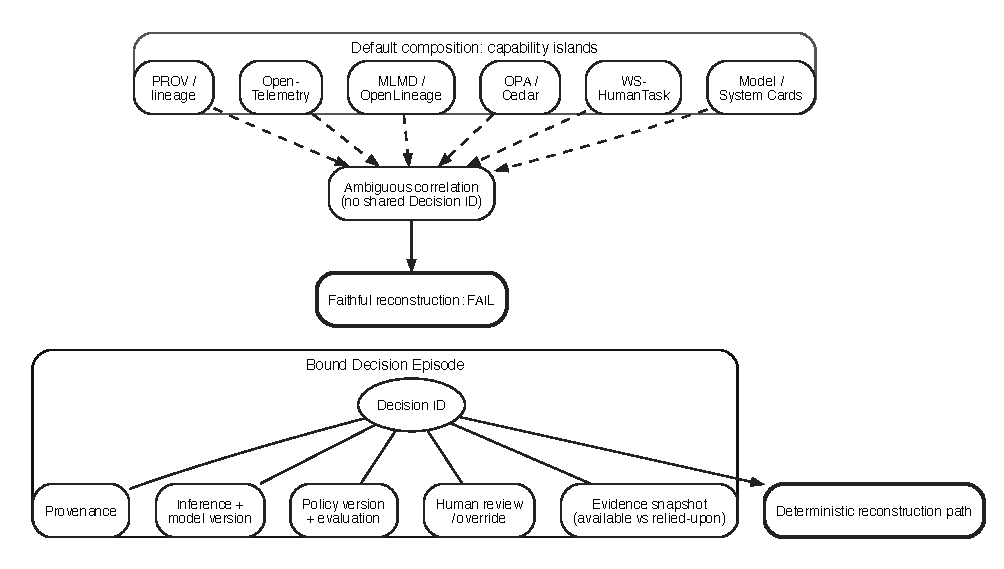
\includegraphics[width=\textwidth]{figures/fig2-fragmented-islands.pdf}
\caption{Left/default: provenance, observability, lineage, policy, documentation, and human-workflow islands without a shared Decision ID yield ambiguous correlation and reconstruction FAIL. Right: the same families contribute objects under a shared Decision ID with decision-time seals. (Source: \texttt{figures/fig2-fragmented-islands.pdf}.)}
\label{fig:2}
\end{figure*}

Composition analysis identifies the principal limitation as \textbf{missing durable cross-component composition of decision knowledge}, not missing individual logging, provenance, explainability, or human--AI workflow support. Critical missing bindings include:


\begin{enumerate}
\item decision ID $\leftrightarrow$ model inference event (model version, inputs, outputs);
\item decision ID $\leftrightarrow$ criteria/policy evaluation (identity + version/bundle revision + result/path);
\item decision ID $\leftrightarrow$ human task (actor, action, timestamps, override semantics);
\item human task $\leftrightarrow$ actor authority (mandate distinct from task role);
\item decision ID $\leftrightarrow$ evidence snapshot (relied-upon subset, not live store);
\item decision ID $\leftrightarrow$ notification and challenge/appeal records where applicable;
\item decision ID $\leftrightarrow$ later correction/remediation;
\item model version $\leftrightarrow$ dataset and feature pipeline versions;
\item criteria version $\leftrightarrow$ effective-date interval and decision timestamp.
\end{enumerate}

None of these bindings is jointly defined as a normative, durable cross-standard contract by the unit sources reviewed. Table 4 contrasts required composition with ecosystem provision.




\begin{table*}[t]
\centering
\small
\begin{tabularx}{\textwidth}{|X|X|X|X|X|}
\hline
 Source object & Target object & Required relationship & Temporal / identity constraint & If absent \\
 \hline
 \hline
 Decision ID & Model inference event & Episode membership & Same ID; model version sealed & Justification FAIL \\
 \hline
 Decision ID & Criteria/policy evaluation & Governing criteria link & Bundle/version at decision time & Authorization/Validity FAIL \\
 \hline
 Decision ID & Human task / review & Human-gate link & Actor + timestamps & Authorization/Justification FAIL \\
 \hline
 Human task & Actor authority & Mandate $\neq$ task role & Authority validity covers act time & Authorization FAIL \\
 \hline
 Decision ID & Evidence snapshot & As-of inputs & Relied-upon $\subset$ available; capture time & Justification FAIL \\
 \hline
 Decision ID & Notification / appeal & Contestability link & Same ID across systems & Contestation path unbound \\
 \hline
 Decision ID & Correction / remediation & Append-only history & No rewrite of sealed commitment & Historical integrity FAIL \\
 \hline
 Model version & Dataset / feature pipeline & Heritage link & Versions resolvable & Drift interpretation FAIL \\
 \hline
 Criteria version & Effective interval + decision time & Temporal coverage & Interval covers decision/effective time & Validity FAIL (latest-only) \\
 \hline
\end{tabularx}
\end{table*}


\subsection{5.4 Base-triad findings (ecosystem)}

For full-episode reconstruction under the scenario set:


\begin{itemize}
\item \textbf{Authorization:} FAIL compositionally; PARTIAL only for narrow policy-log islands.
\item \textbf{Justification:} FAIL (reliance accounting and decision-bound evidence/reasons absent or unbound).
\item \textbf{Validity:} FAIL (historical criteria and evidence as-of binding absent).
\item \textbf{Faithful reconstruction (base):} FAIL.
\end{itemize}

Architecturally, the failures cluster into identity fragmentation; version unbound from episode; authority and human-gate gaps; semantic thinness of purpose-based logs; explanations detached from decision-time packages; provenance without decision context; and challenge pathways that do not key technical episode artefacts. Temporal composition is especially fragile: criteria changes, model replacement, dataset and feature evolution, role changes, personnel turnover, deleted evidence, and regenerable explanations each incentivize latest-only substitution unless decision-time seals exist.


This is an architectural interpretation of the evaluation, not a claim that no organization can invent private integration schemas. Undocumented custom bindings fall outside what the reviewed sources guarantee and outside what the checklist permits as faithful reconstruction without a declared composition.



\subsection{5.5 Reference composition (worked systems profile)}

The compositional FAIL above diagnoses missing \emph{bindings}, not missing \emph{components}. To show that the residual is architecturally actionable, we state a \textbf{reference composition}---a feasibility-oriented systems profile for Scenario 1 (model-assisted eligibility denial). It is \textbf{not} a deployed implementation, \textbf{not} an empirical evaluation, and \textbf{not} evidence that real systems already satisfy the requirements. It answers whether one Decision Episode can be populated from existing families under explicit integration conventions.


\textbf{Narrative.} An eligibility recommendation is produced by a model runtime; a human reviewer accepts it in a workflow system; a policy engine evaluates governing criteria; months later a reconstructor asks for justification, authorization, and temporal validity.


\begin{table*}[t]
\centering
\small
\begin{tabularx}{\textwidth}{|X|X|X|X|X|X|}
\hline
 Component & Contributes object & Populates Decision Episode field & Required binding & If binding omitted & Native vs integration convention \\
 \hline
 \hline
 Inference runtime & AI Inference + outputs & Inference; outcome contribution & Decision ID $\leftrightarrow$ inference event & Justification FAIL & Native inference; \textbf{convention} for Decision ID attribute \\
 \hline
 Model registry / MLMD & Model Version (+ optional dataset/pipeline) & Model/dataset/pipeline versions & Inference $\leftrightarrow$ Model Version; Decision ID $\leftrightarrow$ versions & Drift falsifies historical justification & Native version ids; \textbf{convention} to attach Decision ID \\
 \hline
 Provenance / lineage (PROV or OpenLineage) & Derivation graph / job lineage & Provenance/lineage context & Decision ID $\leftrightarrow$ PROV/lineage root & Derivation unbound to episode & Native graphs; \textbf{convention} for Decision ID as entity/attribute \\
 \hline
 Policy engine (OPA) & Evaluation result + bundle revision & Policy Version; evaluation & Decision ID $\leftrightarrow$ policy decision / bundle revision & Authorization/Validity island only or FAIL & Native decision logs; \textbf{convention} to key by Decision ID \\
 \hline
 Identity / authority source & Human Actor; Authority intervals & Actors; Authority & Review $\leftrightarrow$ Authority; Decision ID $\leftrightarrow$ actors & Authorization FAIL (role$\neq$mandate) & Org IAM native; \textbf{convention} to record authority object at act time \\
 \hline
 Evidence store + snapshotter & Evidence Snapshot & available / relied-upon refs & Decision ID $\leftrightarrow$ snapshot; capture-before-mutation & Justification FAIL & Live store native; \textbf{snapshot+reliance} is integration \\
 \hline
 WS-HumanTask (or equivalent) & Human Review / Override & Review action; optional rationale & Decision ID $\leftrightarrow$ task; task input $\leftrightarrow$ inference hash & Human gate unbound & Native task IDs; \textbf{convention} for Decision ID + required rationale \\
 \hline
 Append-only / immutable episode store & Decision record; sealed bindings & Decision object; seal & All mandatory associations retained & Reconstruction non-deterministic & Not supplied as shared standard; \textbf{composition profile} store \\
 \hline
 Decision ID service & Immutable Decision ID & IC-01 join key & Propagated to all emitters at/before commitment & Scenario 5 FAIL & Application-level convention \\
 \hline
 Reconstruction query API & Published procedure & Triad statements + gaps & Read-only resolve by Decision ID & Heuristic correlation & Profile-defined; fail-closed \\
 \hline
\end{tabularx}
\end{table*}

\textbf{Decision ID propagation.} Mint Decision ID at commitment (or earlier at recommendation acceptance); write it into inference attributes, OPA decision log external key, HumanTask input, evidence snapshot metadata, and PROV entity attributes.


\textbf{Decision-time version bindings.} Seal OPA bundle revision, model hash/version, and evidence snapshot content hashes to the Decision record at commitment; forbid latest-only reads at reconstruction.


\textbf{Reconstruction query.} Given Decision ID, retrieve Decision, Evidence Snapshot, Policy Version+evaluation, Inference+Model Version, Human Review+Authority; evaluate triad; emit explicit gaps if any mandatory binding is missing.


This profile uses only families already reviewed. The residual gap is therefore \textbf{representational and contractual} (shared identity + seals + reliance), not the absence of logging, provenance, policy, or workflow products.



The results motivate an engineering derivation: if the missing capability is durable decision-knowledge representation with semantic bindings, then a solution must reify decision episodes and seal decision-time relationships. Section 6 presents that derived solution.




\subsection{Reference implementation in AIGov}

Section~5.5 argued that the residual gap is architecturally actionable under explicit integration conventions. We next report a \textbf{reference implementation}---AIGov---that \emph{instantiates} selected representational objects from that profile in a real AI-governance infrastructure. AIGov is an audit-backed backend for AI deployments: typed evidence ingest, write-time policy enforcement, append-only hash-chained storage, deterministic compliance projections, and exportable audit artefacts, with an optional parallel AI decision flight recorder.

\paragraph{Purpose (exclusive).}
The implementation has one purpose only: to demonstrate that heterogeneous infrastructure \emph{can preserve} representational objects of the kind required for historical decision reconstructability. It is \textbf{not} intended as independent validation of the Knowledge Continuity Model, \textbf{not} a proof of checklist completeness, and \textbf{not} empirical confirmation of superiority over alternative representations. It demonstrates \textbf{implementation feasibility}, not correctness of the theory. External validation remains future work.

\paragraph{Architecture overview.}
AIGov does not use the product vocabulary ``Decision Episode'' or ``KCM.'' We map paper concepts onto AIGov terminology. The primary unit of decision-bound retention is an evidence \texttt{run\_id}. Authoritative decision-state projection is \texttt{GET /compliance-summary?run\_id=\ldots}, yielding \texttt{VALID}, \texttt{INVALID}, or \texttt{BLOCKED}. Historical retention uses an append-only, hash-chained evidence ledger plus export and integrity-check procedures. A parallel flight recorder retains operational traces (including model version and prompt hash, not raw prompts) and does not replace the compliance-summary projection.

\begin{table*}[t]
\caption{Mapping from paper concepts to AIGov instantiation (feasibility mapping, not a completeness claim).}
\label{tab:aigov-map}
\centering
\scriptsize
\begin{tabularx}{\textwidth}{|X|X|X|X|X|}
\hline
Concept (paper) & AIGov realization & Persisted object & Historical purpose & If absent \\
\hline
Decision Episode & Evidence run as unit & \texttt{run\_id} + events & Bound one decision process & No stable join key \\
\hline
Shared Decision ID & \texttt{run\_id} (+ optional runtime \texttt{decision\_id}) & Run identity & Cross-event membership & Identity fragmentation \\
\hline
Decision knowledge & Typed events + summary & Event sequence; compliance-summary & Retain process facts & Incomplete or \texttt{BLOCKED} \\
\hline
Justification structure & Required justification on human/risk events & Review payloads; evaluation events & Retain stated grounds & Gate incomplete \\
\hline
Authorization snapshot & Write-time policy; approver fields & Policy evaluation; \texttt{human\_approved} & Required acts under policy & \texttt{BLOCKED} \\
\hline
Temporal/version context & \texttt{policy\_version}; model version ids & Version fields & Avoid latest-only substitution & Version ambiguity \\
\hline
Evidence/policy/model bindings & Events keyed by \texttt{run\_id}; version fields & Ledger + pins & Same-identity membership & \texttt{BLOCKED} / unbound model \\
\hline
Prompt bindings & Flight \texttt{prompt\_hash} & Trace start payload & Integrity without raw prompts & Text not retained \\
\hline
Human decision events & \texttt{human\_approved}, \texttt{risk\_reviewed}, \texttt{human\_gate} & Typed events & Human-gate acts & \texttt{BLOCKED} when required \\
\hline
Immutable preservation & Append-only hash-chained ledger & Ledger / traces & Tamper-evident retention & Broken chain \\
\hline
Reconstruction procedure & Export + integrity check + compliance-summary (+ optional flight-pack) & Audit export; summary JSON & Later recovery & No dedicated \texttt{/reconstruct} route \\
\hline
Fail-closed behaviour & Missing required evidence $\Rightarrow$ \texttt{BLOCKED} & \texttt{missing\_evidence} & Refuse silent success & Heuristic success rejected \\
\hline
\end{tabularx}
\end{table*}

\paragraph{Lifecycle.}
A representative lifecycle for one historically retained decision process is: (1)~decision request / activity begins and obtains or creates a \texttt{run\_id}; (2)~identity establishment (\texttt{run\_id} as join key); (3)~policy resolution under the active \texttt{policy\_version}; (4)~authorization / gate resolution (required human/risk event types); (5)~model selection / recording via model-version fields; (6)~evidence collection via \texttt{POST /evidence} under write-time checks; (7)~decision execution / projection via \texttt{GET /compliance-summary}; (8)~sealing / historical storage (append-only hash-chained artefacts); (9)~later reconstruction via export/integrity-check/summary for the same \texttt{run\_id}.

\paragraph{Reconstruction walkthrough.}
Consider a model-promotion gate scoped to AIGov's deployment-governance setting. Request: for \texttt{run\_id}=R, what decision knowledge is retained? Lookup~\texttt{R} in the tenant ledger; retrieve preserved artefacts (export and optional flight-pack); resolve recorded policy and model version pins; resolve same-identity bindings and hash-chain integrity; recover justification fields from retained events; check that required \texttt{human\_approved}/risk-review events exist; use sealed version pins rather than the currently deployed bundle alone; return the compliance-summary projection and supporting exported events. No latency, storage-cost, or accuracy metrics are claimed.

\paragraph{Fail-closed example.}
If policy requires \texttt{human\_approved} but only model/evaluation events exist for~\texttt{R}, \texttt{GET /compliance-summary} yields \texttt{BLOCKED} with structured \texttt{missing\_evidence}/\texttt{blocked\_reasons}. Export may still return the partial chain, but the authoritative projection does not become \texttt{VALID}. Historical reconstruction of a successful authorized decision is therefore unavailable for the missing authorization component; the system does not fabricate approval. This follows the paper's fail-closed representational requirements: absence of a mandatory object yields non-success, not heuristic completion.

\paragraph{Implementation versus evaluation.}
(1)~Analytical evaluation: ecosystem base triad \textbf{FAIL}. (2)~KCM internal coverage: \textbf{PASS under assumptions} (not independent confirmation). (3)~AIGov feasibility: selected objects can be instantiated. AIGov does \textbf{not} independently validate checklist completeness, KCM correctness, or superiority over alternatives. Independent implementations remain future work.


\section{Derived Solution: Knowledge Continuity Model}

The preceding sections identify a missing AI representational capability and evaluate existing approaches against requirements derived from that problem. We now \textbf{derive} an engineering solution implied by the formalization. The Knowledge Continuity Model (KCM) is presented as a consequence of the analysis---not as an independently motivated headline architecture.


KCM elevates the \textbf{Decision Episode} as a representational abstraction for preserving historically meaningful AI decisions. It is a technology-neutral knowledge-representation and composition proposal: persistent objects, semantic bindings, and a reconstruction procedure over historical decision state. It does not mandate a store, ledger, graph database, message bus, or vendor stack. Existing AI-systems components remain valuable; KCM specifies how their outputs can be bound into reconstructable decision knowledge. Alternative compositions that realize the same representational requirements would address the same problem; KCM is one explicit derivation.


\subsection{6.1 Design principles}

The design principles follow from the evaluation diagnosis rather than from a prior product concept: the Decision Episode is the unit of representation; every episode has a stable semantic identity usable across systems; cross-component associations must be explicit and retained, not inferred; reconstruction uses historical structure rather than runtime or latest-only truth; criteria, authorities, models, and evidence carry temporal validity relative to decision time; references point to immutable version identifiers or content hashes; human actors, authority, review acts, overrides, and reasons are first-class decision knowledge; reconstruction preserves the minimal sufficient normative and evidential basis rather than requiring bit-exact replay; the model remains technology-neutral; and adoption can be incremental by binding existing AI components into episodes without replacing them.


\subsection{6.2 Decision Episode as representational abstraction}

\begin{figure*}[t]
\centering
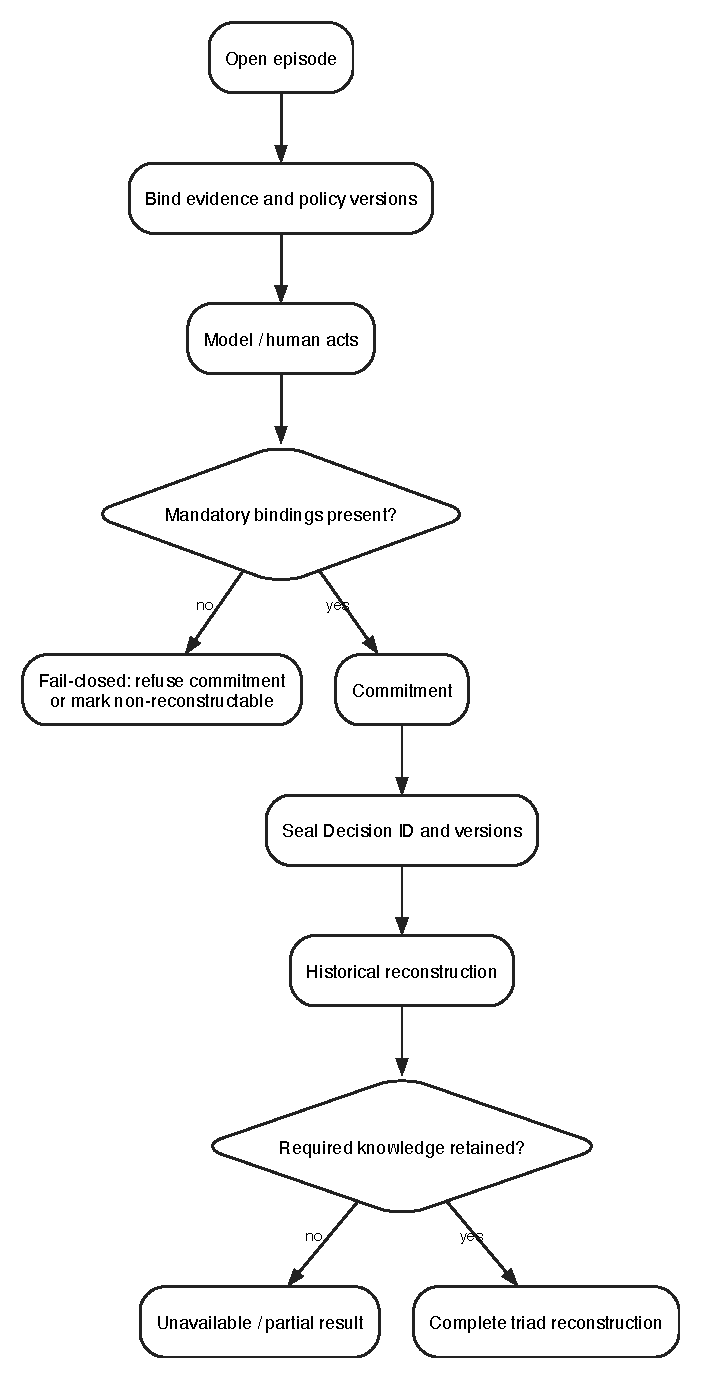
\includegraphics[width=\textwidth]{figures/fig3-decision-episode-lifecycle.pdf}
\caption{Decision Episode lifecycle: open $\rightarrow$ bind evidence/policy $\rightarrow$ acts $\rightarrow$ commitment $\rightarrow$ seal $\rightarrow$ reconstruction, with fail-closed outcomes when mandatory knowledge is missing. (Source: \texttt{figures/fig3-decision-episode-lifecycle.pdf}.)}
\label{fig:3}
\end{figure*}

A \textbf{Decision Episode} is the bounded set of facts, versions, bindings, and acts associated with one decision identity at decision time, plus subsequent review, challenge, and correction acts that refer to that identity. It is a \textbf{representational abstraction} for historically meaningful AI decisions---not a governance workflow construct. In boundary are the commit to an action or controlled outcome in which AI outputs materially participated; the evidence and criteria then treated as applicable; human interventions that produced or altered the outcome; and notices, challenges, and corrections referencing the episode. Out of boundary are unrelated telemetry, later training runs not referenced by the episode, organization-wide criteria repositories except via versioned references, and live feature stores except via evidence snapshots.


Each episode has a single immutable \textbf{Decision ID}, minted at or before commitment, never reused, used as the join key for all bindings, and stable across later correction. Mutable business keys may alias the Decision ID but must not replace it. Lifecycle phases include formation, commitment, disclosure, contest, correction, and retention under a declared profile.


As a KR construct, the Decision Episode is the reified decision state over which later reasoning---explanation retrieval, drift analysis, responsibility attribution, multi-agent handoff review---can operate without recomputing from live models.


\subsection{6.3 Persistent objects as decision knowledge}

\begin{figure*}[t]
\centering
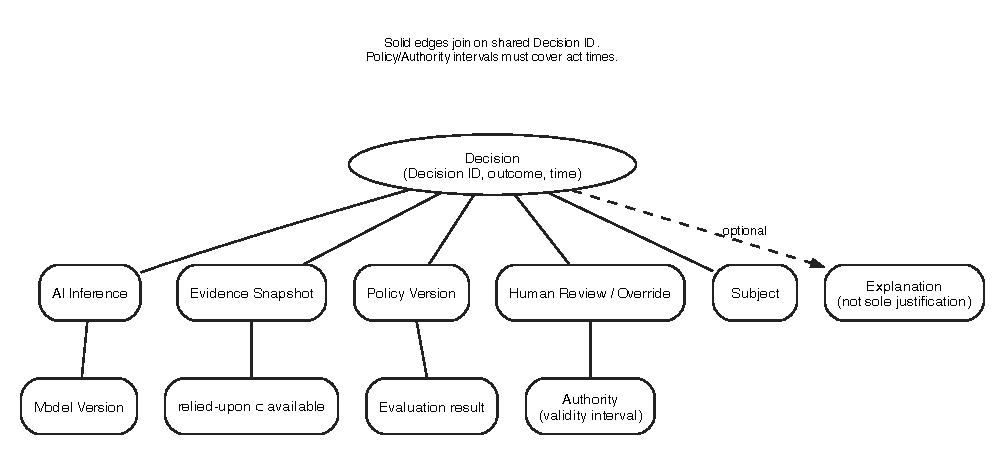
\includegraphics[width=\textwidth]{figures/fig4-kcm-objects-bindings.pdf}
\caption{Principal KCM objects and mandatory relationships: shared Decision ID; relied-upon evidence; authorization with validity intervals; decision-time policy and model version bindings. (Source: \texttt{figures/fig4-kcm-objects-bindings.pdf}.)}
\label{fig:4}
\end{figure*}

KCM defines conceptual persistent objects (attributes are information requirements, not schemas), including: \textbf{Decision} (identity, outcome, decision time, clock domain, status, profile); \textbf{Subject}; \textbf{Human Actor} and \textbf{Organization}; \textbf{Authority} with validity intervals; \textbf{AI Inference}; \textbf{Model Version}, \textbf{Dataset Version}, and \textbf{Feature Pipeline Version}; \textbf{Evidence Snapshot} distinguishing available, relied-upon, and optionally excluded evidence; \textbf{Policy} and \textbf{Policy Version} with validity intervals and evaluation results; \textbf{Explanation} as a decision-time account that is never the sole justification record; \textbf{Human Review} and \textbf{Override} (with required rationale when humans affect the outcome); \textbf{Notification}, \textbf{Appeal}, and \textbf{Remediation}; and optional \textbf{Audit Record} objects for integrity-elevated profiles.


These objects jointly encode representations of decisions, justification, authority, historical context, and temporal validity. Their co-presence without bindings is insufficient; their bound co-presence is the representational claim of KCM.


\subsection{6.4 Semantic bindings}

Bindings are defined exactly once and associate episode objects to the Decision ID (and selected intra-episode associations such as Review $\leftrightarrow$ Authority and Inference $\leftrightarrow$ Model Version). After commitment, associations and referenced version identifiers are immutable; corrections append new objects rather than rewriting history. Absence of a mandatory binding yields reconstruction failure rather than silent guesswork---the operational counterpart of checklist binding criteria, and the mechanism that preserves \textbf{semantic relationships} among decision-knowledge elements.


\subsection{6.5 Temporal model}

KCM distinguishes decision time, effective time, inference time, review time, notification time, appeal time, remediation time, and reconstruction time. Policy versions and authorities carry validity intervals that must cover the relevant act times. Evidence snapshots record capture/as-of time. Correction history is append-only: the original Decision remains, and remediation or a superseding Decision references the original identity. Retaining only current criteria, model, features, explanations, or roles as the sole source of truth is treated as a reconstruction failure mode. This is a model of \textbf{temporal decision knowledge}, not of bi-temporal databases as such---any storage technology may implement the intervals.


\subsection{6.6 Reconstruction procedure}

\begin{figure*}[t]
\centering
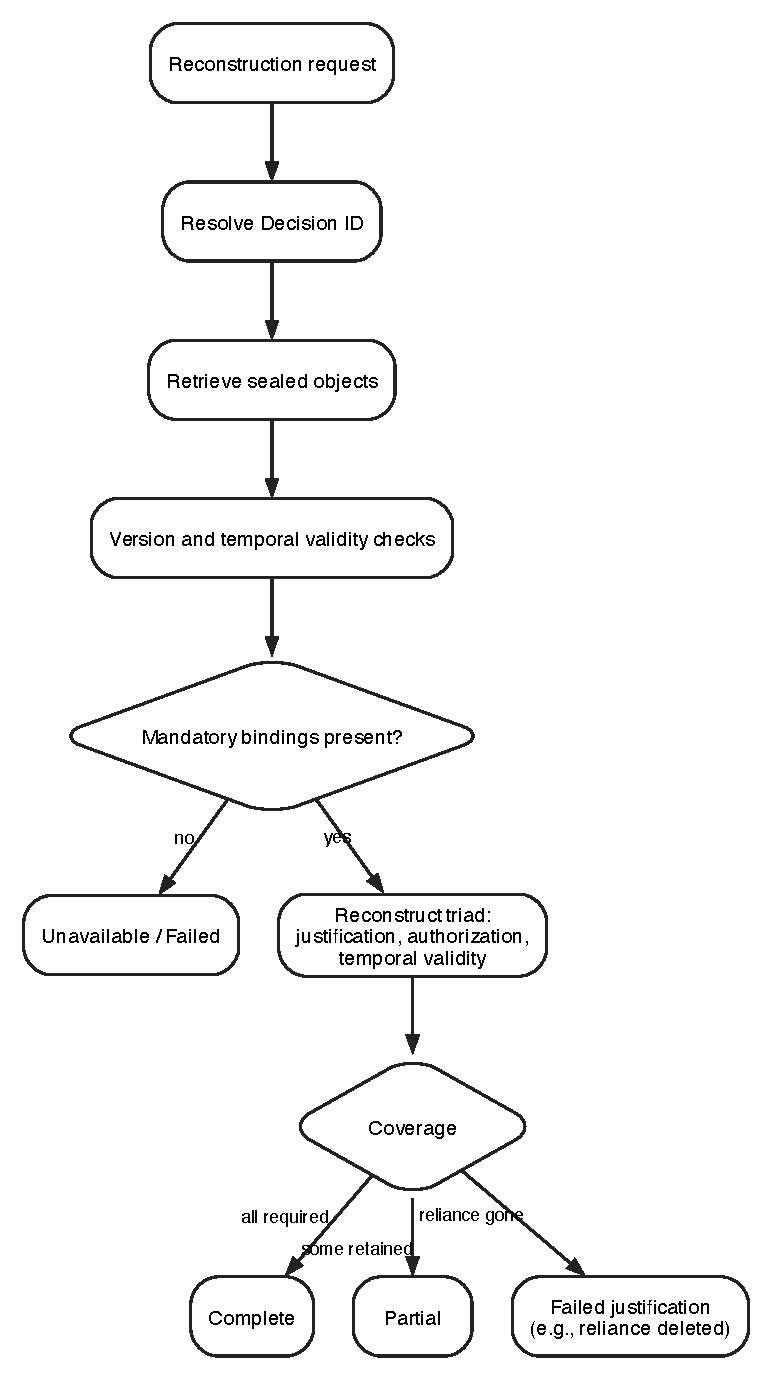
\includegraphics[width=\textwidth]{figures/fig5-reconstruction-process.pdf}
\caption{Reconstruction request resolves a Decision ID, retrieves sealed objects, checks versions and temporal validity, then emits complete, partial, or unavailable triad results---never inventing missing mandatory evidence. (Source: \texttt{figures/fig5-reconstruction-process.pdf}.)}
\label{fig:5}
\end{figure*}

Given a Decision ID, reconstruction resolves the Decision; recovers evidence, criteria version and evaluation, inference, model/dataset/pipeline versions, human acts, authorities, optional explanation, and ordered notification/appeal/remediation records; then evaluates the triad, emitting explicit gaps if mandatory bindings are missing. The procedure is logical rather than executable code; conforming implementations must preserve fail-closed behaviour on missing mandatory bindings. Conceptually, reconstruction is \textbf{reasoning over retained historical decision state}, not re-inference against live models.


\subsection{6.7 How the proposal addresses the gap}

Where the ecosystem fails by unbound islands, KCM requires a shared Decision ID and sealed bindings. Where Scenario 2 fails by latest criteria substitution, KCM seals Policy Version. Where Scenario 3 fails by outcome-only retention, KCM requires Override records with rationale and authority. Where Scenario 4 fails by drift, KCM seals model/dataset/pipeline versions and evidence snapshots. Where Scenario 5 fails by correlation heuristics, KCM forbids reconstruction by undocumented identity guessing. Where Scenario 6 collides with deletion, KCM does not override external deletion constraints; it makes retention and redaction semantics explicit and allows partial reconstruction when only digests or categories remain.



\section{Derived Conformance Specification}

A problem formalization that cannot be tested invites purely rhetorical adoption claims. From the reconstruction requirements and Decision Episode representation we derive a Conformance Specification: how an independent evaluator determines whether an implementation preserves sufficient decision knowledge for deterministic faithful reconstruction. The specification is technology-neutral: it mandates neither storage engines, cryptography, schemas, serialization formats, network protocols, vendor APIs, nor deployment topologies. Normative keywords follow RFC 2119. Conformance evaluates reconstruction capability of a representation; it is not presented as a regulatory certification scheme.


\subsection{7.1 Conformance classes}

\textbf{KC Core} is the minimum class for claiming Knowledge Continuity reconstruction capability for the base triad profile. \textbf{KC Extended} requires Core conformance plus additional requirements that improve robustness, contestability linkage, and integrity-oriented reconstruction. Conformity claims must name the class and declared checklist profile. Vendor-specific profile names are out of scope. Future conformance classes are reserved but not defined. Table 5 summarizes classes and requirement themes.




\begin{table*}[t]
\centering
\small
\begin{tabularx}{\textwidth}{|X|X|X|X|X|}
\hline
 Class & Mandatory capabilities & Optional / Extended & Reconstruction guarantee & Explicit non-guarantees \\
 \hline
 \hline
 KC Core & Decision ID/Episode; outcome/time; historical evidence + reliance distinction; policy version linkage + evaluation; inference/model(/pipeline) linkage; human review/override + authority when applicable; temporal validity; fail-closed published procedure; cross-system bindings (KC-01… applicable Core) & Integrity/signatures; excluded-evidence accounting; contestability extras & Base-triad reconstructability \emph{if} mandatory objects populated and retained & Decision quality/fairness; adoption; bit-exact replay; override of deletion law \\
 \hline
 KC Extended & All Core & Contestability linkage; integrity-oriented Audit Records; additional robustness obligations & Core guarantee plus Extended profile obligations when claimed & Same non-guarantees; Extended does not imply universal completeness \\
 \hline
\end{tabularx}
\end{table*}


\subsection{7.2 Normative requirements (summary)}

The specification assigns stable identifiers KC-01 through KC-34. Requirements cover, among other themes: Decision identity and Episode existence; stable semantic identity; historical evidence and criteria preservation; criteria version and AI inference linkage; model, dataset, and feature-pipeline version linkage; human review and override linkage; authority preservation; temporal validity; explanation, notification, appeal, and remediation linkage; correction history; immutable historical references; cross-system bindings; minimal reconstruction completeness; technology neutrality; published reconstruction procedure; fail-closed behaviour; and subject linkage. Extended-class requirements address additional contestability and integrity-oriented obligations (including audit-oriented records and excluded-evidence accounting where claimed). We do not reproduce all thirty-four requirement blocks here; each block in the authoritative specification states a normative clause, rationale, related checklist items, related KCM principles, conformance class, and verification method (for example document inspection, metadata inspection, historical reconstruction, record traceability, version validation, temporal validation, or graph consistency).


\subsection{7.3 Reconstruction verification}

Successful reconstruction is defined with required inputs (Decision ID, published procedure, retained stores), minimum expected outputs (identity/outcome/time, triad statements, bound object identifiers, explicit gaps), acceptable uncertainty bounds, failure conditions, and historical consistency constraints. The specification distinguishes \textbf{complete}, \textbf{partial}, and \textbf{failed} reconstruction. Missing mandatory bindings yield failure rather than heuristic completion.


\subsection{7.4 Base-triad verification}

Objective pass criteria are stated for Authorization, Justification, and Validity. Authorization requires recoverable actor (as applicable), temporally valid authority, and criteria version/evaluation bound to the same Decision ID. Justification requires evidence snapshot with reliance distinction, inference/model (and pipeline when applicable) linkage, and human rationales when humans affect the outcome; unbound post-hoc explanation is insufficient as sole basis. Validity requires criteria temporal coverage, evaluation/outcome consistency, and prohibition of latest-only substitution. Base faithful reconstruction passes only if all three pass.


\subsection{7.5 Relationship to the checklist and existing infrastructure}

Requirements trace to KCM principles and to checklist categories. The specification complements provenance, observability, lineage, metadata, policy engines, authorization, documentation, explainability, human--AI workflow records, and organizational AI guidance. It does not replace them. Conformance evaluates \textbf{reconstruction capability of a representation}, not regulatory certification.



\section{Evaluation of the Derived Solution}

We evaluate the derived Knowledge Continuity Model analytically with the same checklist marks, base-triad roll-up, and six scenarios used for existing sources. Scoring credits objects and bindings the model defines; it does not credit hypothetical extras, organizational willingness to adopt, or bit-exact replay.


Four claims must be kept distinct:


\begin{enumerate}
\item \textbf{Ecosystem finding.} Reviewed infrastructure families do not compose by default into faithful historical decision reconstruction (Section 5; triad \textbf{FAIL}).
\item \textbf{Construction finding.} KCM was derived to cover the representational requirements identified from that analysis (Sections 3 and 6).
\item \textbf{Internal coverage finding.} Under stated population and preservation assumptions, KCM instantiates those requirements (triad \textbf{PASS} under assumptions). This is an \textbf{internal consistency and requirement-coverage} analysis---evidence that the derived model covers the requirements from which it was constructed---not independent empirical confirmation of sufficiency, not proof of operational feasibility, not proof that the checklist is complete, and not comparative superiority over all alternative models.
\item \textbf{Unresolved external-validation question.} Whether the model is sufficient and practical in deployed systems remains open.
\end{enumerate}

KCM remains PASS only under its stated assumptions; the ecosystem triad remains FAIL.


\subsection{8.1 Checklist evaluation}

Under the base triad profile, KCM systematically supports decision identity, outcome, and time; actors; authority with validity intervals; governing criteria and criteria version; applicable-rule/evaluation path digests when multi-rule policies are in scope; evidence used and evidence relied upon; model version and confidence gates; temporal context; and decision-bound provenance/lineage via versioned bindings. These are the categories on which unit SUTs most often failed compositionally---especially shared identity, criteria-version sealing, and reliance distinction.


Remaining \textbf{PARTIAL} marks arise where the model provides expressibility without a first-class dedicated object, or where the checklist class is optional/conditional: constraints as distinct from criteria/evaluation content; excluded evidence unless elevated; prompts, tools, and external services via snapshot payloads rather than dedicated objects; explicit assumptions structure; jurisdictional frame objects; and integrity/signatures for elevated profiles. These partials are limitations of systematic coverage, not hidden passes.


\subsection{8.2 Base triad}

Under conformant population of mandatory objects and bindings:


\begin{itemize}
\item \textbf{Authorization:} PASS --- actors, temporally valid authority, and sealed criteria version/evaluation on the same Decision ID.
\item \textbf{Justification:} PASS --- evidence snapshot with reliance distinction, bound inference/model context, and human rationales when applicable; post-hoc unbound explanations excluded as sole basis.
\item \textbf{Validity:} PASS --- historical criteria interval coverage and evaluation/outcome consistency without latest-only substitution.
\item \textbf{Faithful reconstruction (base):} PASS under stated assumptions (internal coverage; not external validation).
\item \textbf{Elevated integrity profiles:} PARTIAL until integrity/signature objects are populated.
\end{itemize}

\subsection{8.3 Scenario evaluation}

Table 3 contrasts prior ecosystem results with KCM under conformance. Scenarios 1--5 yield complete base reconstruction when mandatory objects are populated and Decision IDs are propagated; Scenarios 3 and 5 fail if organizations retain outcome-only records or refuse shared identity---those deployments are non-conformant rather than counterexamples to the model's information requirements. Scenario 4 passes for historical justification context without claiming compute-identical replay. Scenario 6 is complete, partial, or failed depending on whether relied-upon evidence remains retained (possibly redacted): redacted snapshots with explicit reliance semantics may preserve partial justification; wholesale destruction of relied-upon evidence without a substitute representation fails justification.


Reconstruction is deterministic under the model's assumptions when bindings are present: the procedure does not rely on undocumented correlation. Determinism here refers to structural triad statements from retained bindings, not to identical floating-point model internals.


\subsection{8.4 Strengths and remaining limitations}

\textbf{Strengths (coverage).} Relative to the gap characterized in Section 5, the derived model \emph{expresses} Decision Episode identity, sealed versions, reliance distinction, human-act/rationale records, authority intervals, and fail-closed reconstruction as first-class decision knowledge. Section 5.5 shows an architectural path to populate those objects from existing components. Neither point is field proof.


\textbf{Remaining limitations.} The model does not solve organizational adoption; incomplete retention; external deletion constraints; evidence never captured; implementation defects; or the substantive quality or optimality of decisions. Category thinness remains for constraints as first-class objects, excluded-evidence accounting, prompt/tool/external-service objects, systematic assumptions structure, jurisdictional-context objects, and integrity/signature elevation. Retroactive stitching of pre-adoption logs without Decision IDs remains non-deterministic. Rationale \emph{quality} is out of scope even when rationale fields are mandatory. Universal completeness is not claimed. Sufficiency is relative to checklist base triad under stated assumptions: mandatory objects populated at commitment, historical version artefacts resolvable, retention horizon honoured, and reconstruction fail-closed on gaps.



\section{Discussion}

\subsection{9.1 The scientific object is the problem}

The central result of this paper is not that a particular model exists, but a refined formulation and systematic characterization of a representational deficiency of contemporary AI systems: they preserve execution while under-preserving the decision knowledge required for faithful historical reconstruction (Figure 1; Tables 1--4). Characterizing that deficiency---its distinction between execution artefacts and decision knowledge; its base triad of justification, authorization, and temporal validity; its reliance and binding conditions; and its compositional evaluation across infrastructure families---is the principal AI contribution. Adjacent KR traditions (§2.8) motivate episode and temporal structure without substituting for cross-component bindings. The reference composition (§5.5; Figure 2) shows architectural actionability without claiming deployment proof. The AIGov reference implementation (\S5.6) further shows that selected representational objects can be \emph{instantiated} in a working system; that demonstration addresses practical implementability and does \textbf{not} eliminate the need for external validation, comparative evaluation, or empirical deployment studies. Engineering artefacts (checklist, KCM, conformance; Figures 3--5; Table 5) are instruments of that characterization and one derived response, evaluated only for internal coverage (Section 8).


\subsection{9.2 Why the problem grows with future AI systems}

As AI systems become longer-lived, more compositional, and more entangled with other agents and tools, the interpretive distance between \emph{current execution state} and \emph{past committed decisions} increases. Assistants accumulate commitments; orchestrators chain tools; multi-agent systems redistribute evidence and authority; autonomous systems update controllers while past acts remain consequential. None of these trends was experimentally measured here. They indicate, without speculation about particular products, that the historical decision reconstruction problem is unlikely to shrink as AI systems scale in duration and composition. Governance and regulated settings will continue to expose the deficiency; they do not exhaust it.


\subsection{9.3 Implications for AI systems and knowledge representation}

For knowledge representation, AI systems, agents, multi-agent systems, decision support, and long-lived deployments that commit to outcomes with lasting interpretive significance, preserving decision knowledge---identity, justification structure, authority, temporal validity, and semantic bindings---belongs among first-order representation requirements, not among optional telemetry hygiene. The analytical evaluation suggests that investing solely in more logs, richer provenance graphs, or better explanation interfaces will not reliably produce historical reconstruction if those artefacts remain unbound to a decision identity and to decision-time versions. \textbf{Decision knowledge} is a distinct representational layer relative to execution knowledge; provenance remains a relevant substrate that can encode portions of that knowledge without guaranteeing compositional reconstructability.


\subsection{9.4 Potential application domains}

We did \textbf{not} experimentally validate the following domains; we identify them as natural settings in which the formalized problem is likely to arise:


\begin{itemize}
\item \textbf{Decision-support systems}, where recommendations become commitments and must remain interpretable after model updates.
\item \textbf{AI assistants and long-lived agents}, where cumulative commitments, tool uses, and user confirmations form an evolving decision history.
\item \textbf{AI orchestration and multi-step workflows}, where bindings must span planners, tools, and downstream actuators.
\item \textbf{Multi-agent systems}, where justification and authority cross agent boundaries and informal correlation of messages is insufficient.
\item \textbf{Autonomous systems}, where post-incident reconstruction must recover decision-time criteria and evidence rather than current controller parameters.
\item \textbf{Human--AI collaborative systems}, where overrides and rationales are part of the decision representation, not optional comments.
\end{itemize}

Regulated eligibility and oversight settings remain important \emph{stress tests} of the same representational requirements.


\subsection{9.5 Incremental adoption of the derived solution}

Where organizations choose to address the formalized gap using KCM's derivation, an adoption path begins by minting and propagating a Decision ID at the commitment point; wrapping existing policy-engine results, model-registry versions, and workflow completions as bound objects; adding evidence snapshotting beside live feature access; enforcing commitment gates that reject incomplete mandatory bindings; and extending to notification and challenge systems where applicable. Early steps do not require replacing OPA, OpenTelemetry, HumanTask processors, or model registries. AIGov (\S5.6) illustrates one such path using \texttt{run\_id}-keyed append-only evidence and fail-closed projections, without claiming that path is the only or complete realization of KCM.


\subsection{9.6 Relationship to existing AI tooling}

The formalized requirements complement provenance, observability, lineage/metadata, policy engines, authorization languages, documentation, explainability, and human--AI workflow records. Those components continue to provide derivation, paths, pipeline versions, evaluation semantics, release descriptions, explanation quality, and task lifecycle. What they do not jointly define---and what the problem statement demands---is episode membership with sealed decision-time semantic relationships and fail-closed reconstruction over historical decision state.


\subsection{9.7 Trade-offs}

Evidence snapshots cost storage and raise tension with data minimization; Scenario 6 shows that deletion of relied-upon inputs can force partial or failed justification even when other logs survive. Commitment gates increase operational friction but prevent silent non-conformance. Minimal sufficient reconstruction deliberately excludes bit-exact replay, which lowers forensic ambition while matching the checklist's adequacy threshold. Elevated integrity (checksums, signatures) strengthens trustworthiness of retained records but is not required for base content faithfulness.


\subsection{9.8 Scope and generality}

The historical decision reconstruction problem, as formalized here, concerns reconstruction capability of decision knowledge. It does not assess decision quality, fairness, security hardening, or organizational process maturity. It is stated at a level of generality independent of law and compliance. Domain profiles may elevate optional checklist categories without weakening Required items.


What would count as addressing the problem without adopting KCM as a product is any declared composition that realizes the same Decision Episode representational requirements, publishes a reconstruction procedure, and fails closed on missing mandatory associations. Such a composition would confirm the \emph{problem formalization}; it would not erase the finding that the reviewed sources do not already define those bindings.


\subsection{What the reference implementation does and does not settle}

AIGov reduces one practical concern raised by systems readers: whether the residual semantic-binding gap is merely descriptive. By operationalizing shared run identity, append-only retention, version pins, human-gate justifications, export/integrity-check procedures, and fail-closed \texttt{BLOCKED} outcomes, the reference implementation shows implementability of selected requirements. It does \textbf{not} settle external validation of the checklist, comparative evaluation against alternative episode models, or empirical studies of deployment frequency and cost. Those remain open.



\section{Threats to Validity}

\textbf{Conceptual evaluation.} Ecosystem and KCM scores assess specified information models and analytical scenarios, not measured frequencies in industry deployments. Adoption claims are accordingly constrained.


\textbf{Implementation dependence.} Optional features in sources (for example optional HumanTask comments, Cedar without a log sink) widen capability ceilings but not guarantees. Similarly, KCM triad PASS depends on commitment gates and retention; implementation failure falsifies a deployment, not the checklist alignment of the specification text.


\textbf{Publication and corpus bias.} The corpus privileges published primary sources selected for family coverage. Unpublished organizational schemas might already realize episode bindings. Such a schema would be a successful \emph{composition profile} realizing KCM-like requirements; it would not show that the reviewed standards already define those bindings.


\textbf{Domain dependence.} Narrow application-specific logging fields must not be generalized into a complete decision representation. Profiles may need domain adaptation.


\textbf{Future standards.} Future AI-systems standards or profiles may later standardize the same bindings under other names. The finding concerns the reviewed ecosystem at the evaluation's source pins, not perpetual impossibility.


\textbf{Alternative composition mechanisms.} The evaluation does not assert that only a branded new product layer can succeed. A composition profile over existing stores that realizes the same objects and bindings would also satisfy the information requirements. Authoring bias is a further threat because KCM was derived to answer composition failures; mitigation consists in using the same checklist and scenarios, and in recording PARTIAL marks and Scenario 6 limits explicitly.


\textbf{Absence of deployment measurements.} Scenarios are adversarial structural tests. They show failure modes consistent with unit boundaries; they do not estimate how often organizations already invent adequate private integrations.


\textbf{Circular evaluation risk.} Because KCM was designed against the checklist, Section 8 is an internal coverage check under conformance assumptions, not independent field efficacy and not external validation of sufficiency. We treat that limitation as intrinsic to conceptual KR evaluation at this stage and state it as claim (3) versus unresolved claim (4) in Section 8.


\textbf{Author-developed reference implementation.} AIGov is developed by the authors. It therefore cannot constitute independent validation of the theory, the checklist, or KCM. Its reported role is solely to demonstrate that selected representational requirements are \emph{implementable} in a working AI-governance infrastructure. Independent third-party implementations, blinded replications of the analytical marks, and deployment measurements remain future work.



\section{Conclusion}

Contemporary AI systems preserve execution. They do not, on the evidence of our analytical evaluation of representative infrastructure, adequately preserve the decision knowledge required for deterministic faithful historical reconstruction of justification, authorization, and temporal validity. We refined and characterized that gap as the \textbf{historical decision reconstruction problem}---an Artificial Intelligence knowledge-representation and systems problem that exists independently of law, regulation, governance, and compliance.


Contributions follow a fixed hierarchy: (1)~refined problem formulation; (2)~representational requirements for historical decision knowledge; (3)~unit and compositional evaluation of contemporary AI infrastructure; (4)~identification of the residual semantic-binding and shared-identity gap; (5)~the derived Knowledge Continuity Model and Conformance Specification centred on the Decision Episode abstraction; and (6)~a reference implementation (AIGov) demonstrating that selected representational objects can be instantiated in a working system. Under stated assumptions an internal coverage analysis finds that the derived model satisfies base-triad requirements (PASS under assumptions)---not empirical proof of deployment sufficiency. The reviewed ecosystem composition remains FAIL for the base triad; adoption, retention, evidence deletion, and several conditional categories remain limiting. The AIGov demonstration addresses implementability only; it does not independently validate the theory.


The principal scientific contribution is therefore refined problem formulation and systematic characterization---previously under-characterized in this specific representational and compositional form---and distinguishable from logging, provenance formats, workflow engines, and explainability methods, while acknowledging provenance and DEMM as related but non-subsuming work. The engineering model and reference implementation are derived instruments of that contribution; the implementation does not elevate above the scientific contribution and remains replaceable by any composition that realizes the same representational requirements.


Future work includes alternative compositions that realize the formalized requirements without a distinct product layer; domain-specific profile elevations; studies of reconstructability in multi-agent and long-lived assistant settings; deployment measurements; and integrity-elevated reconstructions. Those steps should reuse the Reconstruction Checklist rather than weaken the problem characterization.




\bibliographystyle{plainnat}
\bibliography{library}


\appendix
\section{JAIR Reproducibility Checklist (submission appendix)}
\label{app:repro}

\noindent\textit{This appendix is required for JAIR review. Answers reflect the analytical character of this manuscript. Authors must confirm answers against the official JAIR Author Kit checklist wording before portal upload.}

\begin{itemize}
\item \textbf{Claims type:} Conceptual / analytical characterization and standards-based evaluation; not a learning-system empirical study.
\item \textbf{Code:} Reference implementation (AIGov) reported as feasibility demonstration only; not an empirical evaluation artefact. Figure sources provided.
\item \textbf{Data:} No training/evaluation dataset collected. Evaluation uses published primary sources listed in unit reviews; artefacts available in repository path \texttt{topics/ai-infrastructure-gap/}.
\item \textbf{Experimental setup:} Analytical unit reviews, scenario analysis, and composition analysis; scoring rules in review methodology and reconstruction checklist v0.1.0.
\item \textbf{Randomness / seeds:} Not applicable.
\item \textbf{Compute:} Not applicable (no model training).
\item \textbf{Human subjects:} Not applicable.
\item \textbf{Limitations:} Stated in Section~Threats to Validity and evaluation framing (internal coverage vs external validation).
\item \textbf{Reproducibility of scores:} Given the same primary sources, checklist version, and methodology document, another analyst can re-apply marks; some PARTIAL judgments involve interpretive reading of standards text.
\end{itemize}

\textit{Note:} Replace this appendix with the filled official JAIR template checklist when the Author Kit is applied.

\end{document}
